\documentclass[11pt]{article}
\usepackage[T1]{fontenc}
\usepackage[a4paper,margin=25mm,headheight=14pt]{geometry}
\usepackage{amsmath,amssymb,amsthm,graphicx,booktabs,xcolor}
\usepackage{microtype}
\usepackage{caption}
\usepackage{hyperref}
\definecolor{ink}{HTML}{172E43}
\definecolor{teal}{HTML}{007F8B}
\hypersetup{colorlinks=true,linkcolor=teal,citecolor=teal,urlcolor=teal,
  pdftitle={Replication-induced instability of a certified five-cluster motor cycle}}
\captionsetup{font=small,labelfont=bf,labelsep=period}
\setlength{\parskip}{.35em}
\setlength{\parindent}{1em}
\setlength{\emergencystretch}{2em}
\newtheorem{theorem}{Theorem}
\newtheorem{proposition}[theorem]{Proposition}
\newtheorem{corollary}[theorem]{Corollary}
\newcommand{\spec}{\operatorname{spec}}
\newcommand{\diag}{\operatorname{diag}}
\newcommand{\Id}{\mathrm{I}}
\newcommand{\R}{\mathbb R}
\newcommand{\repo}{\href{https://github.com/Griboedow/chaos-attractor-lab}{\texttt{chaos-attractor-lab}}}
\title{\color{ink}Replication-induced instability of a\\certified five-cluster motor cycle}
\author{}
\date{30 October 2026\quad\textbullet\quad Pre-submission manuscript}
\begin{document}
\maketitle
\vspace{-1.5em}
\begin{abstract}
An exactly repeated collective motion need not retain its stability when its
constituent groups are enlarged. We give a computer-assisted example in the
first-harmonic molecular-motor model of Alouges and collaborators. At explicit
parameters, an eight-row system has an attracting periodic orbit with five
distinct cluster states and multiplicities $2+2+1+2+1$. Interval integration,
multiple shooting and spectral tests certify its existence and place all
22 nonflow Floquet multipliers inside modulus $0.13$. Exact replication to
$N=8k$ rows preserves the orbit and the cluster weights, but gives precisely
$2k-2$ unstable, one neutral and $22k$ stable directions. The instability is
carried by internal differences in the two groups that were singletons at
$N=8$. Each newly available block has one real multiplier in
$(-23.084,-23.083)$ and two multipliers of modulus below $0.13$.
The proof combines an explicit invariant splitting with reproducible interval
certificates. Full-system numerical trajectories illustrate attraction and
sign-reversing departure without serving as premises of the theorem.
\end{abstract}
\noindent\textbf{Keywords:} cluster synchronization; periodic orbit;
Floquet stability; molecular motors; validated numerics.

\section{Introduction}
Collective oscillations are often represented by a small collection of
distinct group states. Such a description retains the motion within the
cluster subspace but can hide perturbations that split an individual group.
This distinction becomes consequential when a small configuration is
replicated: the same group trajectories may survive exactly while new
internal degrees of freedom make them unstable.

Alouges et al.~\cite{alouges} introduced a model for interactions between
rows of molecular motors in an axonemal cross-section. Their eight-row
numerical examples display periodic motion organized into two groups;
the organization of the general $3N-1$ dimensional system is left open.
We study an explicit five-cluster cycle in its exact first-harmonic
specialization. The question is whether attraction of this motion survives
balanced enlargement of every cluster.

Symmetry-based separation of cluster motion and transverse perturbations is
established in synchronization theory~\cite{pecora,sorrentino}. Connections
between different cluster patterns, symmetry breaking and chaos have also
been studied in globally coupled oscillators~\cite{haugland}. Our
contribution is an explicitly enclosed orbit and a complete stability
classification of its replicated family in the motor equations. The
proof resolves every tangent direction, including ones absent in the
smallest member of the family.

The central result is that the $N=8$ cycle attracts locally, whereas all
replicas with $N=8k$, $k\geq2$, are saddles. The instability is strong:
a perturbation in each new unstable mode reverses sign and grows in
magnitude by about $23.08$ over a certified return period. This is a
change in the available perturbation space as the system size changes.
The theorem concerns fixed normalized parameters and fixed cluster weights.
It makes no identification of this enlargement with changing the anatomy
of a physical flagellum while holding all dimensional constants fixed.

\section{Model and main result}
For $N\geq2$, write the state of row $j$ as $(c_j,s_j,X_j)$ and impose
$\sum_j X_j=0$. In normalized time $\tau$, the equations are
\begin{align}
 V_j&=-\rho X_j+r(s_j-\bar s),&
 \bar s&=\frac1N\sum_{i=1}^N s_i,\label{eq:velocity}\\
 c_j'&=1-c_j-V_js_j,&
 s_j'&=b-s_j+V_jc_j,& X_j'&=V_j.\label{eq:model}
\end{align}
The first harmonic of the motor density determines $(c_j,s_j)$; $X_j$ is
the normalized relative displacement. Eliminating $X_N$ gives a
$3N-1$ dimensional autonomous polynomial system. The mean term in
\eqref{eq:velocity} follows from the mechanical displacement constraint.
The normalization and its relation to the published equations are given
in the accompanying source audit. This manuscript uses
\begin{equation}
 \rho_* = \frac{129}{55},\qquad
 r_* = 1+\frac{19/20}{\sqrt{32001/500000}},\qquad b_*=1.
 \label{eq:parameters}
\end{equation}
The value of $r_*$ agrees with the activity path implemented from the source
model. The rational value of $\rho_*$ specifies the theorem exactly and
avoids identifying a floating-point grid point with an exact parameter.

\begin{theorem}[Certified cycle and complete replication index]
\label{thm:main}
At \eqref{eq:parameters}, the $N=8$ system has a nonconstant periodic orbit
with five pairwise distinct cluster states and multiplicities
$(m_1,\ldots,m_5)=(2,2,1,2,1)$. It has a positive return period satisfying
\begin{equation}
25.0016843758970971<T<25.0016843758970972.\label{eq:period}
\end{equation}
For every integer $k\geq1$, replication to multiplicities
$(2k,2k,k,2k,k)$ is an exact periodic solution of the $N=8k$ system at
the same parameters and with the same return period. Its Floquet index is
\begin{equation}
 (u,n,s)=(2k-2,\,1,\,22k),\label{eq:index}
\end{equation}
where $u,n,s$ count multipliers outside, on and inside the unit circle,
with algebraic multiplicity. The sole neutral multiplier is the simple
flow multiplier $1$. Every stable multiplier has modulus below $0.13$.
Every unstable multiplier belongs to $(-23.084,-23.083)$.
In particular, the $N=8$ orbit is locally orbitally exponentially attracting;
the $N=8k$ replicas are hyperbolic periodic saddles for $k\geq2$.
\end{theorem}

The theorem certifies a return period. It does not assert that the displayed
$T$ is the least positive period. The stability and index conclusions do
not require such an assertion: taking a positive integer power of a
minimal-period monodromy preserves the numbers of stable and unstable
directions. The simplicity of the flow multiplier is certified for the
displayed return.

\begin{figure}[t]
\centering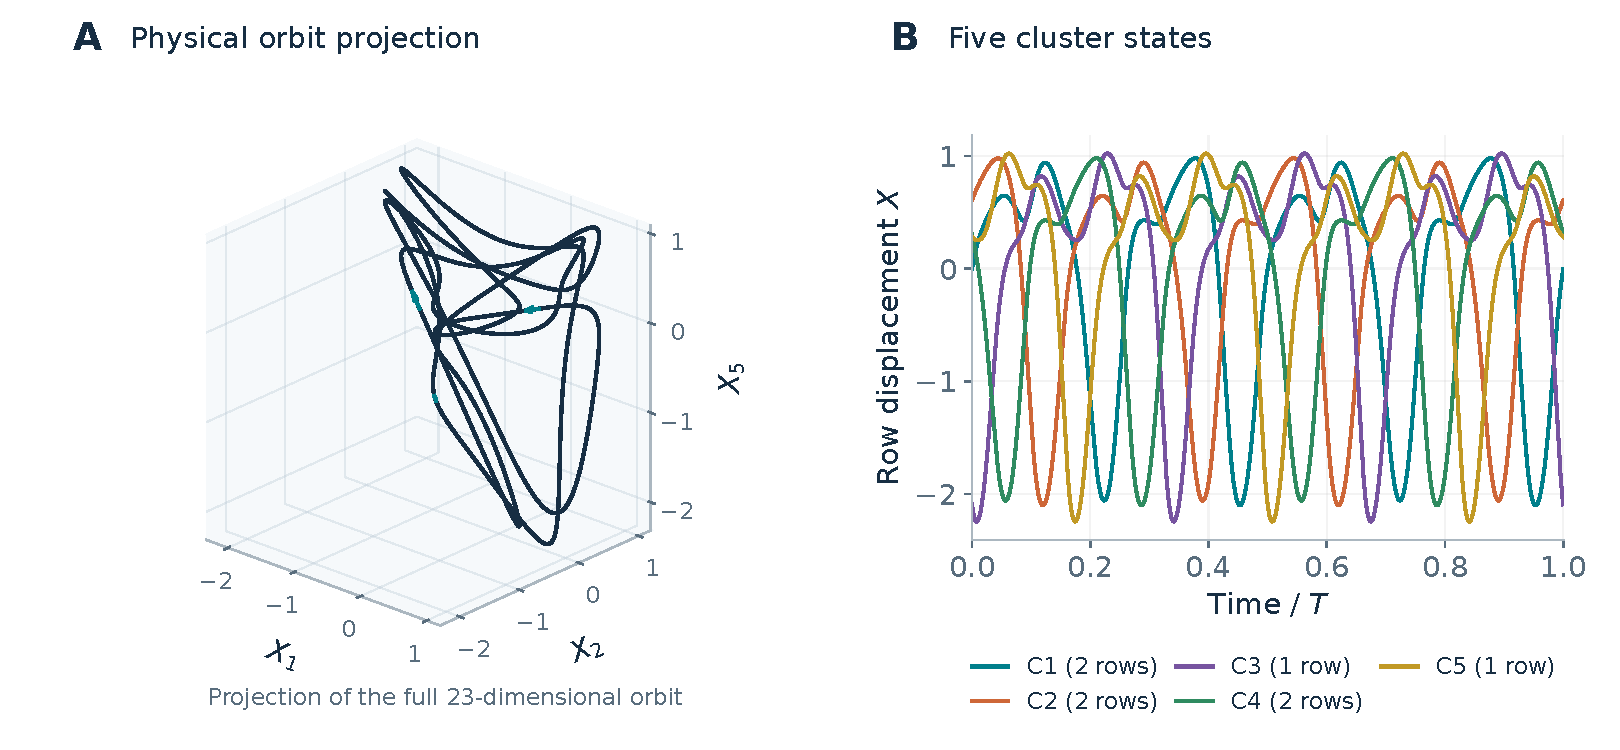
\includegraphics[width=\linewidth]{figures/figure-1-cycle.pdf}
\caption{The certified five-cluster orbit. (A) A numerical rendering in
three physical displacement coordinates; the full state has 23 independent
coordinates. Arrows indicate increasing time. (B) One row displacement
from each distinct cluster over the certified return period, with cluster
sizes in the legend. Geometric closure in panel A is illustrative;
existence follows from interval multiple shooting.}
\label{fig:cycle}
\end{figure}

\section{Invariant splitting and replication}
Partition the rows into $K$ nonempty groups of sizes $m_a$ and write
$w_a=m_a/N$. On the cluster subspace, all rows of group $a$ have the same
state $(c_a,s_a,X_a)$. Substitution in \eqref{eq:velocity}--\eqref{eq:model}
gives the weighted quotient
\begin{equation}
 V_a=-\rho X_a+r\left(s_a-\sum_{b=1}^K w_b s_b\right),
 \qquad \sum_{a=1}^K w_a X_a=0,\label{eq:quotient}
\end{equation}
with the same three row equations. It has dimension $3K-1$.
Multiplying every $m_a$ by the same positive integer leaves all weights
unchanged. Therefore every quotient trajectory, periodic or otherwise,
embeds exactly in every balanced replica.

Along a cluster trajectory, an internal perturbation has zero sum within
one cluster in each of its three coordinates. It changes neither the
global mean of $s$ nor the displacement constraint. Each independent
internal contrast in group $a$ obeys
\begin{equation}
 \xi'=A_a(\tau)\xi,\qquad
 A_a=\begin{pmatrix}
 -1&-V_a-rs_a&\rho s_a\\
 V_a&-1+rc_a&-\rho c_a\\
 0&r&-\rho
 \end{pmatrix}.\label{eq:contrast}
\end{equation}
There are $m_a-1$ such three-dimensional copies. The remaining tangent
directions are constant within each cluster and form the quotient tangent
space. This is a direct sum: decomposing row perturbations into their
cluster averages and zero-sum residuals gives unique components.

\begin{proposition}[Replication spectrum]
\label{prop:splitting}
Let $M_Q$ be the quotient monodromy over a positive period $T$, and let
$M_a$ be the return matrix of \eqref{eq:contrast}, whether or not the
group is a singleton in the original system. The monodromy of the
replica with multiplicities $km_a$ is similar to
\begin{equation}
 M_Q\ \oplus\ \bigoplus_{a=1}^K
      \left(\Id_{km_a-1}\otimes M_a\right).\label{eq:split}
\end{equation}
Equivalently, its characteristic polynomial is
\begin{equation}
 \chi_{8k}(z)=\chi_Q(z)\prod_{a=1}^5\chi_a(z)^{km_a-1}
 \label{eq:polynomial}
\end{equation}
for the five-cluster family considered here.
\end{proposition}
\begin{proof}
The cluster-average and zero-sum spaces described above are invariant
under the variational equation. On each contrast copy the equation is
\eqref{eq:contrast}; on the average space it is the derivative of
\eqref{eq:quotient}. The dimensions sum to
$(3K-1)+3\sum_a(km_a-1)=3kN-1$, so no direction is omitted.
Integration over $T$ preserves the direct sum and gives \eqref{eq:split}.
The determinant factorization yields \eqref{eq:polynomial}.
\end{proof}

For a singleton, $m_a-1=0$. Its matrix $M_a$ describes a mathematically
well-defined response along the orbit, but contributes no direction to
the original tangent space. Replication makes this matrix dynamically
relevant. Consequently attraction at $N=8$ puts no stability restriction
on the two absent singleton blocks. This identifies precisely the
information needed in addition to the original stability certificate.

\section{Computer-assisted proof}
The proof uses outward-enclosing Arb ball arithmetic through Python-FLINT
0.9.0~\cite{arb}. The inclusion argument is a finite-dimensional
verification argument of the type surveyed in~\cite{rump}. The custom
flow integrator, complete inputs, lossless interval outputs and executed
source snapshots are provided in the repository. Ordinary numerical
shooting supplies initial proposals only.

\subsection{Relative periodicity and validated shooting}
Let $q$ denote the 14 independent quotient coordinates, with the last
displacement eliminated using \eqref{eq:quotient}. Define a weight-preserving
permutation by
\begin{equation}
 (Pq)_a=q_{\pi(a)},\qquad \pi=(4,1,5,2,3),\qquad P^6=\Id,
 \label{eq:permutation}
\end{equation}
where the list specifies the image index for each group. The certified
relative closure is $\phi_L(q_0)=Pq_0$ with $L=T/6$.
It cyclically exchanges the three paired groups and swaps the singletons.

We divide $L$ into three equal segments of duration $\ell=L/3$. Unknowns
are $q_0,q_1,q_2$ and $\ell$, with the phase fixed by $X_1(q_0)=0$.
There are 42 free scalar unknowns and 42 equations:
\begin{equation}
 F(q_0,q_1,q_2,\ell)=
 \begin{pmatrix}
 \phi_\ell(q_0)-q_1\\
 \phi_\ell(q_1)-q_2\\
 \phi_\ell(q_2)-Pq_0
 \end{pmatrix}=0.\label{eq:shoot}
\end{equation}
The Jacobian includes the endpoint vector field as the derivative with
respect to duration. A ball $\mathcal B$ around an approximate solution
$\hat q$ and a fixed invertible preconditioner $C$ satisfy
\begin{equation}
 -CF(\hat q)+\bigl(\Id-C[DF(\mathcal B)]\bigr)
       (\mathcal B-\hat q)
       \subset\operatorname{int}(\mathcal B-\hat q).\label{eq:kraw}
\end{equation}
The induced infinity norm of $\Id-C[DF(\mathcal B)]$ is strictly below
one. Thus $q\mapsto q-CF(q)$ is a contraction of the box into itself;
its unique fixed point is a zero of $F$ because $C$ is invertible.
The verified positive section velocity and duration exclude a stationary
solution. Pairwise disjoint coordinate enclosures at the section verify
that all five cluster states are distinct. Uniqueness of the ODE then
prevents any two cluster states from coinciding at another time.

Each flow step first encloses a Picard tube for all uncertain initial
states and durations and checks a contraction bound. The polynomial
Taylor recurrence is then evaluated at the input box; its next-order
coefficient is enclosed over the entire tube to bound the remainder.
The same procedure integrates the variational blocks. Bounds therefore
include truncation, rounding and input uncertainty.

\subsection{Full-space attraction at eight rows}
Write $H=D\phi_L(q_0)$ and $Q=P^{-1}H$. Equivariance gives
\begin{equation}
 M_Q=Q^6.\label{eq:relative}
\end{equation}
The nonzero vector field at the section is an exact eigenvector of $Q$
with eigenvalue one. After an invertible, exactly stored dyadic similarity,
the interval characteristic polynomial is divided by the exact factor
$z-1$. A Schur recursion certifies all 13 remaining roots of $Q$ inside
radius $0.7$. Consequently the 13 nonflow multipliers of $M_Q$ satisfy
$|\mu|<0.7^6=0.117649$.

Let $B_a$ be the return of \eqref{eq:contrast} over the relative interval
$L$, starting from the certified section. The ordered full-period return
for the first paired group is
\begin{equation}
 M_1=(B_2B_4B_1)^2.\label{eq:pairs}
\end{equation}
The other two paired groups use the corresponding cyclic products. Each
of these three enclosed cubic characteristic polynomials passes a Schur
test at radius $0.13$. At $N=8$, these blocks supply nine stable directions.
Together with the quotient, this proves the $(0,1,22)$ index and full-space
local attraction. The spectrum in a restricted cluster subspace alone
would not imply this conclusion.

\subsection{The formerly absent blocks and their exact index}
The two singleton blocks follow the alternating group path $3,5,3,5,3,5$,
so their full returns are
\begin{equation}
 M_3=(B_5B_3)^3,\qquad M_5=(B_3B_5)^3.\label{eq:singleton}
\end{equation}
These matrices are similar because $B_3$ is a fundamental matrix and is
invertible. They therefore have the same spectrum. We nevertheless
enclose and check both separately, retaining the uncertainty in every
matrix product.

For each cubic $p(z)=z^3+a_2z^2+a_1z+a_0$, strict interval signs first
give a real root outside the unit disk. Bisection yields the common
outward-readable bracket
\begin{equation}
 -23.083470<\mu_u<-23.083469.\label{eq:root}
\end{equation}
For an exact root $u$ in this bracket, synthetic division gives
\begin{equation}
 p(z)=(z-u)\left[z^2+\alpha z+\beta\right],\quad
 \alpha=a_2+u,\quad \beta=a_1+u(a_2+u).\label{eq:division}
\end{equation}
All admissible coefficients and roots are enclosed when evaluating
$\alpha$ and $\beta$. For a real monic quadratic, roots lie within radius
$R$ if
\begin{equation}
 1-|\beta|/R^2>0,\qquad
 1+\alpha/R+\beta/R^2>0,\qquad
 1-\alpha/R+\beta/R^2>0.\label{eq:jury}
\end{equation}
These strict inequalities hold at $R=0.13$ for the entire enclosing
coefficient box. Thus each singleton block has exactly one unstable root
and two stable roots. A failed stability test alone would not give this
classification; the root bracket and quadratic inequalities supply it.

In the replica, the paired groups provide $3(2k-1)$ copies of stable
three-dimensional blocks. The two formerly singleton groups provide
$2(k-1)$ copies of blocks with index $(1,0,2)$. Including the quotient,
\begin{align*}
 u&=2(k-1),\qquad n=1,\\
 s&=13+9(2k-1)+4(k-1)=22k.
\end{align*}
This proves Theorem~\ref{thm:main}. All stable block bounds are below
$0.13$, so this same bound holds for every replicated stable multiplier.

\begin{corollary}[Persistence near the certified parameters]
There is an open neighborhood of $(\rho_*,r_*,b_*)$ in which the relative
five-cluster orbit continues and every balanced replica retains the
index \eqref{eq:index}.
\end{corollary}
\begin{proof}
The verified nonsingularity of the shooting Jacobian and the implicit
function theorem continue the relative orbit locally. The weights and
permutation remain fixed. Its quotient and five contrast return matrices
depend continuously on the parameters. All nonflow spectra are separated
strictly from the unit circle. A common sufficiently small neighborhood
therefore preserves the index of these finitely many blocks, and
Proposition~\ref{prop:splitting} gives the statement for every $k$.
\end{proof}
This corollary is qualitative; no numerical radius of the parameter
neighborhood has been validated.

\subsection{Recomputation and quantitative margins}
Table~\ref{tab:validation} separates periodic-orbit validation, new
variational integrations and spectral replay. The original periodic
certificate and its recomputation use the same implementation and arithmetic
library with different precision, subdivision and Taylor settings. They
are not independent proof implementations. Independent field/Jacobian
embeddings and exact rational Taylor-coefficient controls supplement them.

\begin{table}[t]
\centering\small
\begin{tabular}{lrrrl}
\toprule
Calculation & Bits & Steps/segment & Order & Verified conclusion\\
\midrule
Cycle inclusion and spectrum &448&144&48&Attracting $N=8$ cycle\\
Cycle recomputation &512&160&50&Same orbit and sharp bounds\\
Singleton integration &512&160&50&Real unstable roots\\
Singleton reintegration &640&192&54&Same enclosed spectrum\\
Spectral replay (both records)&768&---&---&Exact $(1,0,2)$ block index\\
\bottomrule
\end{tabular}
\caption{Distinct roles of the validated computations. Steps are counted
within each of the three shooting segments. Spectral replay rereads the
complete stored interval matrices and retains their radii.}
\label{tab:validation}
\end{table}

For the 512-bit cycle recomputation, the Krawczyk contraction bound is
below $1.960\times10^{-19}$ and the maximum component inclusion ratio is
below $2.574\times10^{-12}$. The shooting-box radius is $10^{-38}$.
The 640-bit singleton reintegration also passes the independent embedding
check against the full 47-dimensional $N=16$ Jacobian, including the group
containing the eliminated displacement coordinate. There are 1,692 checked
components at rational test states. These algebra controls detect
implementation inconsistencies; the invariant splitting itself is derived
in Section~3.

The quadratic radius-$0.13$ inequalities remain well separated from zero;
their smallest interval lower margin exceeds $0.9999$. Source snapshots,
input hashes, interval matrices and the separate spectral replay are
preserved for both integration settings. The computational proof remains
conditional on the correctness of the stated algorithms, implementation
and arithmetic library; it is not proof-assistant formalization.

\section{Nonlinear numerical illustrations}
The figures use ordinary floating-point integrations of the full
$3N-1$ dimensional equations. They provide geometric and dynamical
interpretation of the certified linear stability. They are not used to
prove the existence of the periodic orbit or its Floquet classification.

\subsection{Approach to the eight-row orbit}
Six starts were declared at phases $jT/6$, $j=0,\ldots,5$, with random
perturbations of full physical-state norm $0.03$. The displacement
perturbations have zero sum, and all three paired groups are initially
split. The fixed random seed and all initial states are retained. No
clustering condition is imposed during the integration.

Distance is measured in all 24 physical coordinates, including the
reconstructed displacement, and minimized numerically over the phase of
the reference orbit. After six periods, all six distances fall from
approximately $0.03$ to between $1.32\times10^{-7}$ and
$3.42\times10^{-7}$ (Fig.~\ref{fig:dynamics}A). Some trajectories first
move farther from the orbit, so local attraction does not imply monotone
decay in this norm. Tightening the DOP853 settings changes any displayed
state by less than $8.62\times10^{-11}$.

These six local examples do not estimate a basin volume or a certified
basin radius. The repository also retains an earlier declared amplitude
$0.6$ set: none of those six starts passed the six-period approach gate,
and five failed long-horizon pointwise solver agreement. Their eventual
destinations are not classified. All amplitudes remain in the data audit.

\begin{figure}[t]
\centering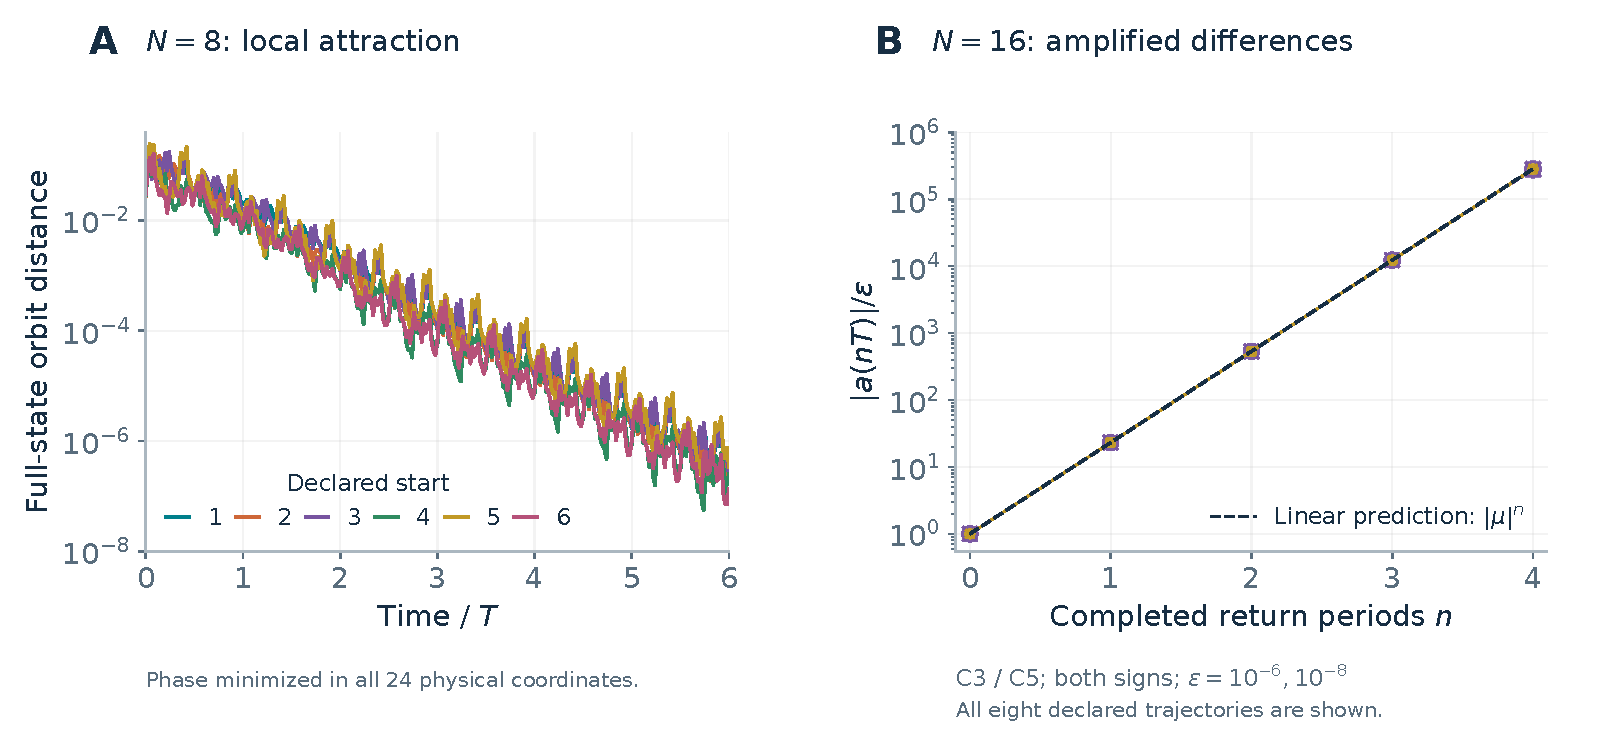
\includegraphics[width=\linewidth]{figures/figure-2-dynamics.pdf}
\caption{Full-system numerical checks of the two stability outcomes.
(A) Every declared nearby $N=8$ trajectory, with numerical phase
minimization in the full physical state. (B) All eight $N=16$ starts:
two newly available contrast blocks, two signs and two perturbation norms.
The signed contrast component $a$ is sampled at $nT$; absolute values are
normalized by the initial norm $\varepsilon$. Solid and dotted curves
correspond to $10^{-8}$ and $10^{-6}$, respectively; circles and crosses
distinguish signs. The dashed line is the linear Floquet prediction.
Overlapping curves are retained.}
\label{fig:dynamics}
\end{figure}

\subsection{Sign-reversing departure at sixteen rows}
We replicate the certified section state to groups of sizes
$(4,4,2,4,2)$. For each formerly singleton group, a numerical eigenvector
$v$ of the midpoint return matrix proposes an unstable direction. Its
two rows receive perturbations $\pm\varepsilon v/\sqrt2$, so the full
physical perturbation has norm $\varepsilon$ and leaves all group means
unchanged at the initial instant. Both overall signs and
$\varepsilon\in\{10^{-6},10^{-8}\}$ give eight declared starts.
The full nonlinear dynamics are integrated for four periods.

For the normalized row contrast
$\xi=(\delta q_a-\delta q_b)/\sqrt2$, let $a=v^\mathsf{T}\xi$.
At small amplitude the stroboscopic prediction is
$a(nT)\simeq a(0)\mu_u^n$. The negative multiplier produces alternation
of sign, while its magnitude gives rapid amplification
(Figs.~\ref{fig:dynamics}B and~\ref{fig:replication}C). For all four
$10^{-8}$ starts, relative discrepancies from this prediction at the first
three returns are below $10^{-6}$. The larger-amplitude starts also remain
in the archived ensemble when nonlinear corrections become visible.

Both DOP853 settings are retained for every trajectory. Their maximum
pointwise state difference is below $2.69\times10^{-8}$. A separate
Radau integration, using the analytic full Jacobian, checks one complete
larger-amplitude history and differs by less than $1.97\times10^{-8}$.
These are finite numerical controls and do not identify the eventual
attractors reached after departure.

\begin{figure}[t]
\centering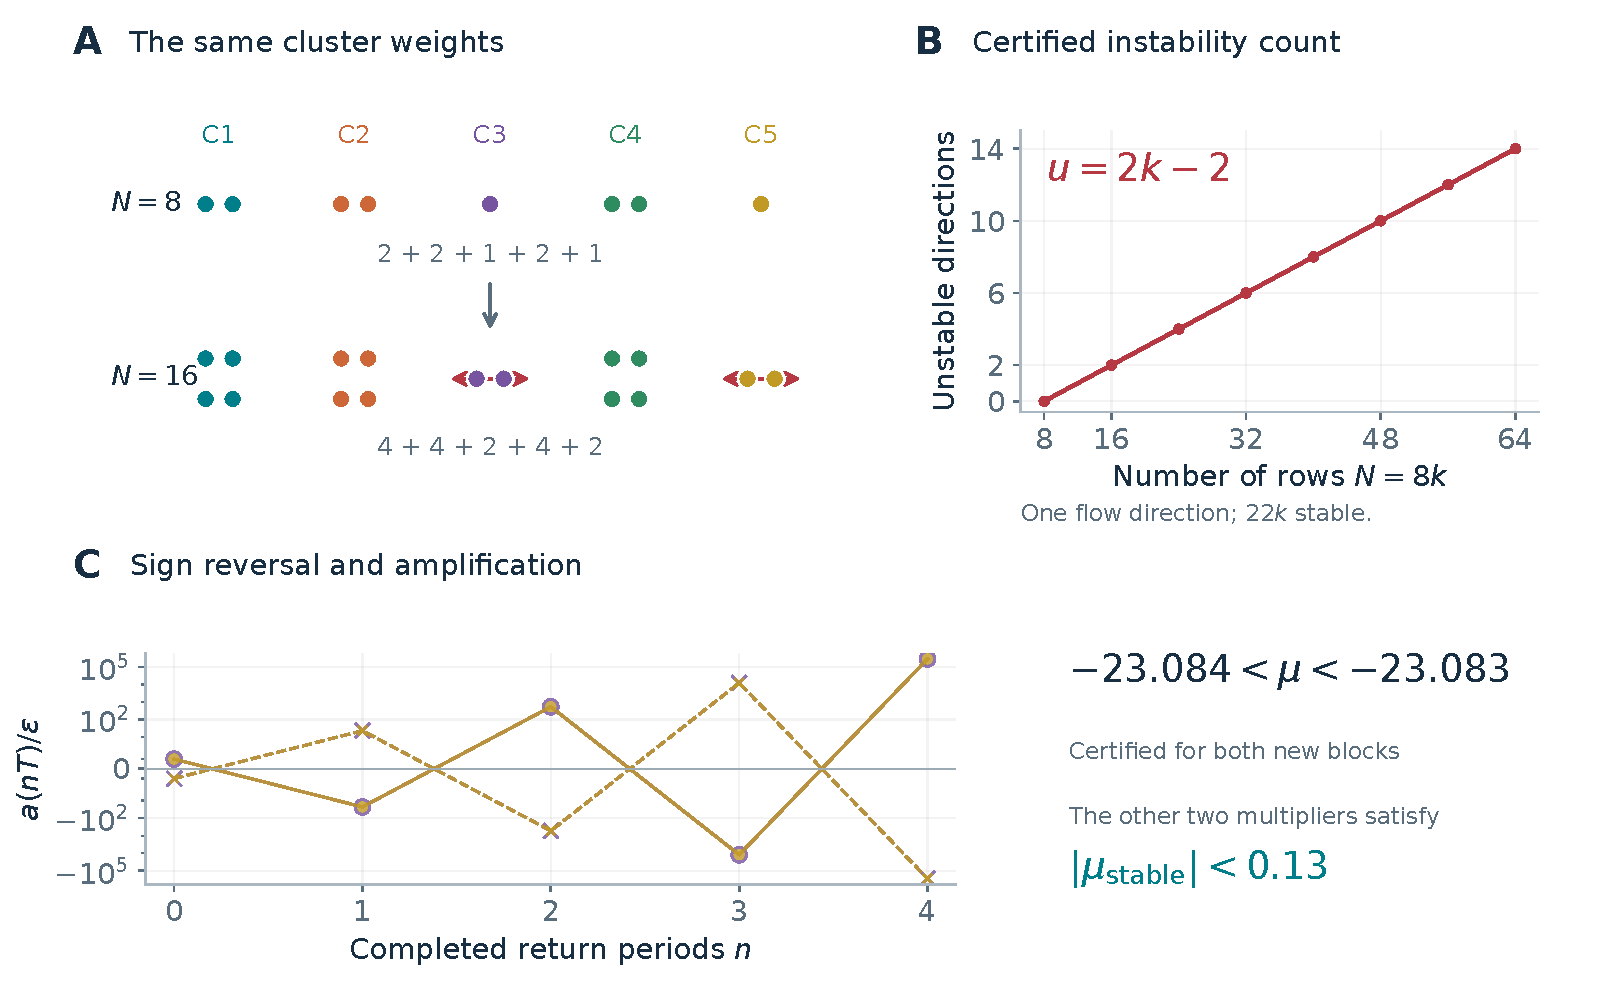
\includegraphics[width=\linewidth]{figures/figure-3-replication.pdf}
\caption{The mechanism and its quantitative consequence. (A) Enlarging
all groups preserves their weights. Red arrows mark new internal
differences in the two original singletons. (B) The exact unstable count
$2k-2$; displayed points are discrete system sizes, and the theorem holds
for every integer $k\geq1$. (C) Both signs in both new blocks at
$\varepsilon=10^{-8}$, shown on a symmetric logarithmic vertical scale.
The displayed multiplier bounds are interval-certified; the return
trajectories are numerical illustrations.}
\label{fig:replication}
\end{figure}

\section{Discussion}
The five-group state supplies a concrete distinction between preserving
a collective motion and preserving its attraction. The quotient orbit
does not change under balanced replication, yet the admissible tangent
space does. Two previously absent blocks become available, and their
unstable multiplier fixes the complete growth in saddle index. Existing
cluster-stability theory provides the organizing framework; the explicit
periodic orbit, interval enclosures and exact index formula establish the
model-specific result.

The bounds also show that the effect is robust to sufficiently small
parameter changes. It does not rely on a multiplier lying close to one
or on a long transient whose classification is uncertain. Quantifying
the parameter neighborhood and locating the nonlinear destinations of
departing replicas are natural extensions.

Separate computations in this model exhibit a candidate regime with six
positive finite-time Lyapunov estimates and very long switching
trajectories. Those results are documented in the repository, but do not
enter the theorem proved here. A connection from the certified cycle or
its replicas to those regimes would require additional global analysis.
The present paper establishes a periodic-attractor and periodic-saddle
result, without an asymptotic chaos claim or a claim of historical
priority for cluster desynchronization as a general mechanism.

\section*{Data and code availability}
The complete materials are available in the \repo\ repository.
The manuscript directory is \path{papers/replication-instability}.
Its README maps claims and figures
to immutable evidence records and gives regeneration commands. The
article manifest supplies raw-byte SHA-256 hashes. The certificate inputs
use lossless dyadic midpoint/radius serialization. All numerical initial
conditions, settings and outcomes are retained. The figures are available
as vector PDF and SVG, with PNG previews and a rotating view whose camera
motion is explicitly distinguished from dynamical evolution.

\appendix
\section{Density interpretation and physical admissibility}
Let $\ell$ be the spatial period, $a_0>0$ the constant total transition
rate, $\kappa$ the elastic stiffness, $\eta$ the drag coefficient and
$U$ the potential amplitude. With dimensional density $Q_j$ and relative
shift $\Delta_j$, the normalization is
\[
 \theta=\frac{2\pi\xi}{\ell},\quad \tau=a_0t,\quad
 q_j=\ell Q_j,\quad X_j=\frac{2\pi\Delta_j}{\ell},\quad
 \rho=\frac{\kappa}{\eta a_0},\quad
 \gamma=\frac{2\pi^2U}{\eta\ell^2a_0}.
\]
For transition-rate Fourier coefficients $a_1,b_1$, put
$A=a_1/a_0$ and $B=b_1/a_0$.
Under a cosine interaction potential, constant total transition rate and
sinusoidal forcing, write the normalized density equation as
\begin{equation}
 \partial_\tau q_j+V_j\partial_\theta q_j
 =-q_j+\frac12+A\cos\theta+B\sin\theta.
\end{equation}
Setting the first Fourier coefficients to $Ac_j$ and $As_j$, with
$b=B/A$ and $r=-\gamma A$, gives \eqref{eq:model}. Only the first sine
coefficient enters the force. Thus this finite system is an exact closure
under the stated assumptions. Higher-mode relaxation is already present
in the source model~\cite{alouges}.

For $b=1$, the row amplitude satisfies
\[
 (c_j^2+s_j^2)'=-2(c_j^2+s_j^2)+2(c_j+s_j).
\]
At a maximum along a periodic solution this implies
$c_j^2+s_j^2\leq2$. Hence the lifted density
$q_j=1/2+A(c_j\cos\theta+s_j\sin\theta)$ is positive whenever
$|A|\sqrt2<1/2$. The source activity-path convention satisfies this
condition at the parameter used here. This statement concerns the
specified density model; a mechanically bending flagellum coupled to
fluid would require additional state variables and analysis.

An omitted Fourier coefficient of order $n\geq2$ evolves as
\[
 z_{j,n}(\tau)=
 e^{-\tau+in[X_j(\tau)-X_j(0)]}z_{j,n}(0).
\]
The omitted mean relaxes at the same exponential rate. Since
$X_j(T)=X_j(0)$, these residual modes have return multiplier $e^{-T}$
and add only stable directions. More directly, the residual density is
an exponentially damped spatial translation; its periodic Sobolev norm
is multiplied exactly by $e^{-\tau}$. This proves local attraction of the
lifted $N=8$ cycle in these norms. The replicas' finite-dimensional
unstable directions persist within the invariant zero-tail subspace.

\section{A compact verification recipe}
The decisive records, all relative to the repository root, are
\begin{enumerate}
\raggedright
\item \path{results/motor-five-cycle-proof/recheck-01.json}: periodic
inclusion, quotient and paired spectra at 512 bits;
\item \path{results/motor-replication-article/reintegration-640.json}:
new singleton return matrices from a 640-bit variational integration;
\item \path{results/motor-replication-article/exact-index-recheck.json}:
strict real-root brackets and quadratic radius tests at 768 bits;
\item \path{results/motor-replication-article/nonlinear/}: the declared
eight-start illustration and a different-solver control.
\end{enumerate}
The new index checker recomputes each cubic from the stored interval
matrix, cross-checks the coefficients with explicit $3\times3$ formulas,
brackets the negative root by strict signs and verifies
\eqref{eq:jury}. It never substitutes a midpoint eigenvalue for an
interval statement. A second replay uses the earlier 512-bit matrices.
Reproduction writes to unused output paths and preserves all earlier
records. The README supplies the separate proof and visualization
dependency sets; the proof requires no GPU, NumPy or SciPy.

\begin{thebibliography}{9}
\raggedright
\bibitem{alouges}
F. Alouges, I. Anello, A. DeSimone, A. Lefebvre-Lepot, and J. Levillain,
Some mathematical models for flagellar activation mechanisms,
\emph{Mathematical Models and Methods in Applied Sciences} \textbf{35}
(2025), 2395--2424.
\href{https://doi.org/10.1142/S0218202525500423}{doi:10.1142/S0218202525500423}.
\href{https://arxiv.org/abs/2409.03506}{arXiv:2409.03506}, version 2.

\bibitem{pecora}
L. M. Pecora, F. Sorrentino, A. M. Hagerstrom, T. E. Murphy, and R. Roy,
Cluster synchronization and isolated desynchronization in complex
networks with symmetries, \emph{Nature Communications} \textbf{5} (2014), 4079.
\href{https://doi.org/10.1038/ncomms5079}{doi:10.1038/ncomms5079}.

\bibitem{sorrentino}
F. Sorrentino, L. M. Pecora, A. M. Hagerstrom, T. E. Murphy, and R. Roy,
Complete characterization of the stability of cluster synchronization in
complex dynamical networks, \emph{Science Advances} \textbf{2} (2016), e1501737.
\href{https://doi.org/10.1126/sciadv.1501737}{doi:10.1126/sciadv.1501737}.

\bibitem{haugland}
S. W. Haugland and K. Krischer,
Connecting minimal chimeras and fully asymmetric chaotic attractors
through equivariant pitchfork bifurcations,
\emph{Physical Review E} \textbf{103} (2021), L060201.
\href{https://doi.org/10.1103/PhysRevE.103.L060201}{doi:10.1103/PhysRevE.103.L060201}.

\bibitem{arb}
F. Johansson, Arb: efficient arbitrary-precision midpoint-radius interval
arithmetic, \emph{IEEE Transactions on Computers} \textbf{66} (2017), 1281--1292.
\href{https://doi.org/10.1109/TC.2017.2690633}{doi:10.1109/TC.2017.2690633}.

\bibitem{rump}
S. M. Rump, Verification methods: rigorous results using floating-point
arithmetic, \emph{Acta Numerica} \textbf{19} (2010), 287--449.
\href{https://doi.org/10.1017/S096249291000005X}{doi:10.1017/S096249291000005X}.
\end{thebibliography}
\end{document}
